\section{Mathematical Methodologies}

...

  \subsection{Point Process}

  ...

     \subsubsection{Introduction}

      ...

     \subsubsection{Survival Function $S(r)$}
     

      ...
      

  \subsection{Monte Carlo Simulation for Stochastic Process}


  ...

    \subsubsection{Heat Content $Q(\tau)$ and Survival Function $S_{\Omega}(\tau)$}

  
    ...



    \subsubsection{Design LRWs in the $2-$ dimensional image}
    
       \begin{itemize}
           \item Initial condition: uniform distribution within $\Omega$, which is bounded by the border of the image and the edge of the target object.
           \item Boundary condition
             \begin{itemize}
               \item Perodic boundary condition the edges of the image.
               \par

               
                 \begin{figure}
                   \centering
                   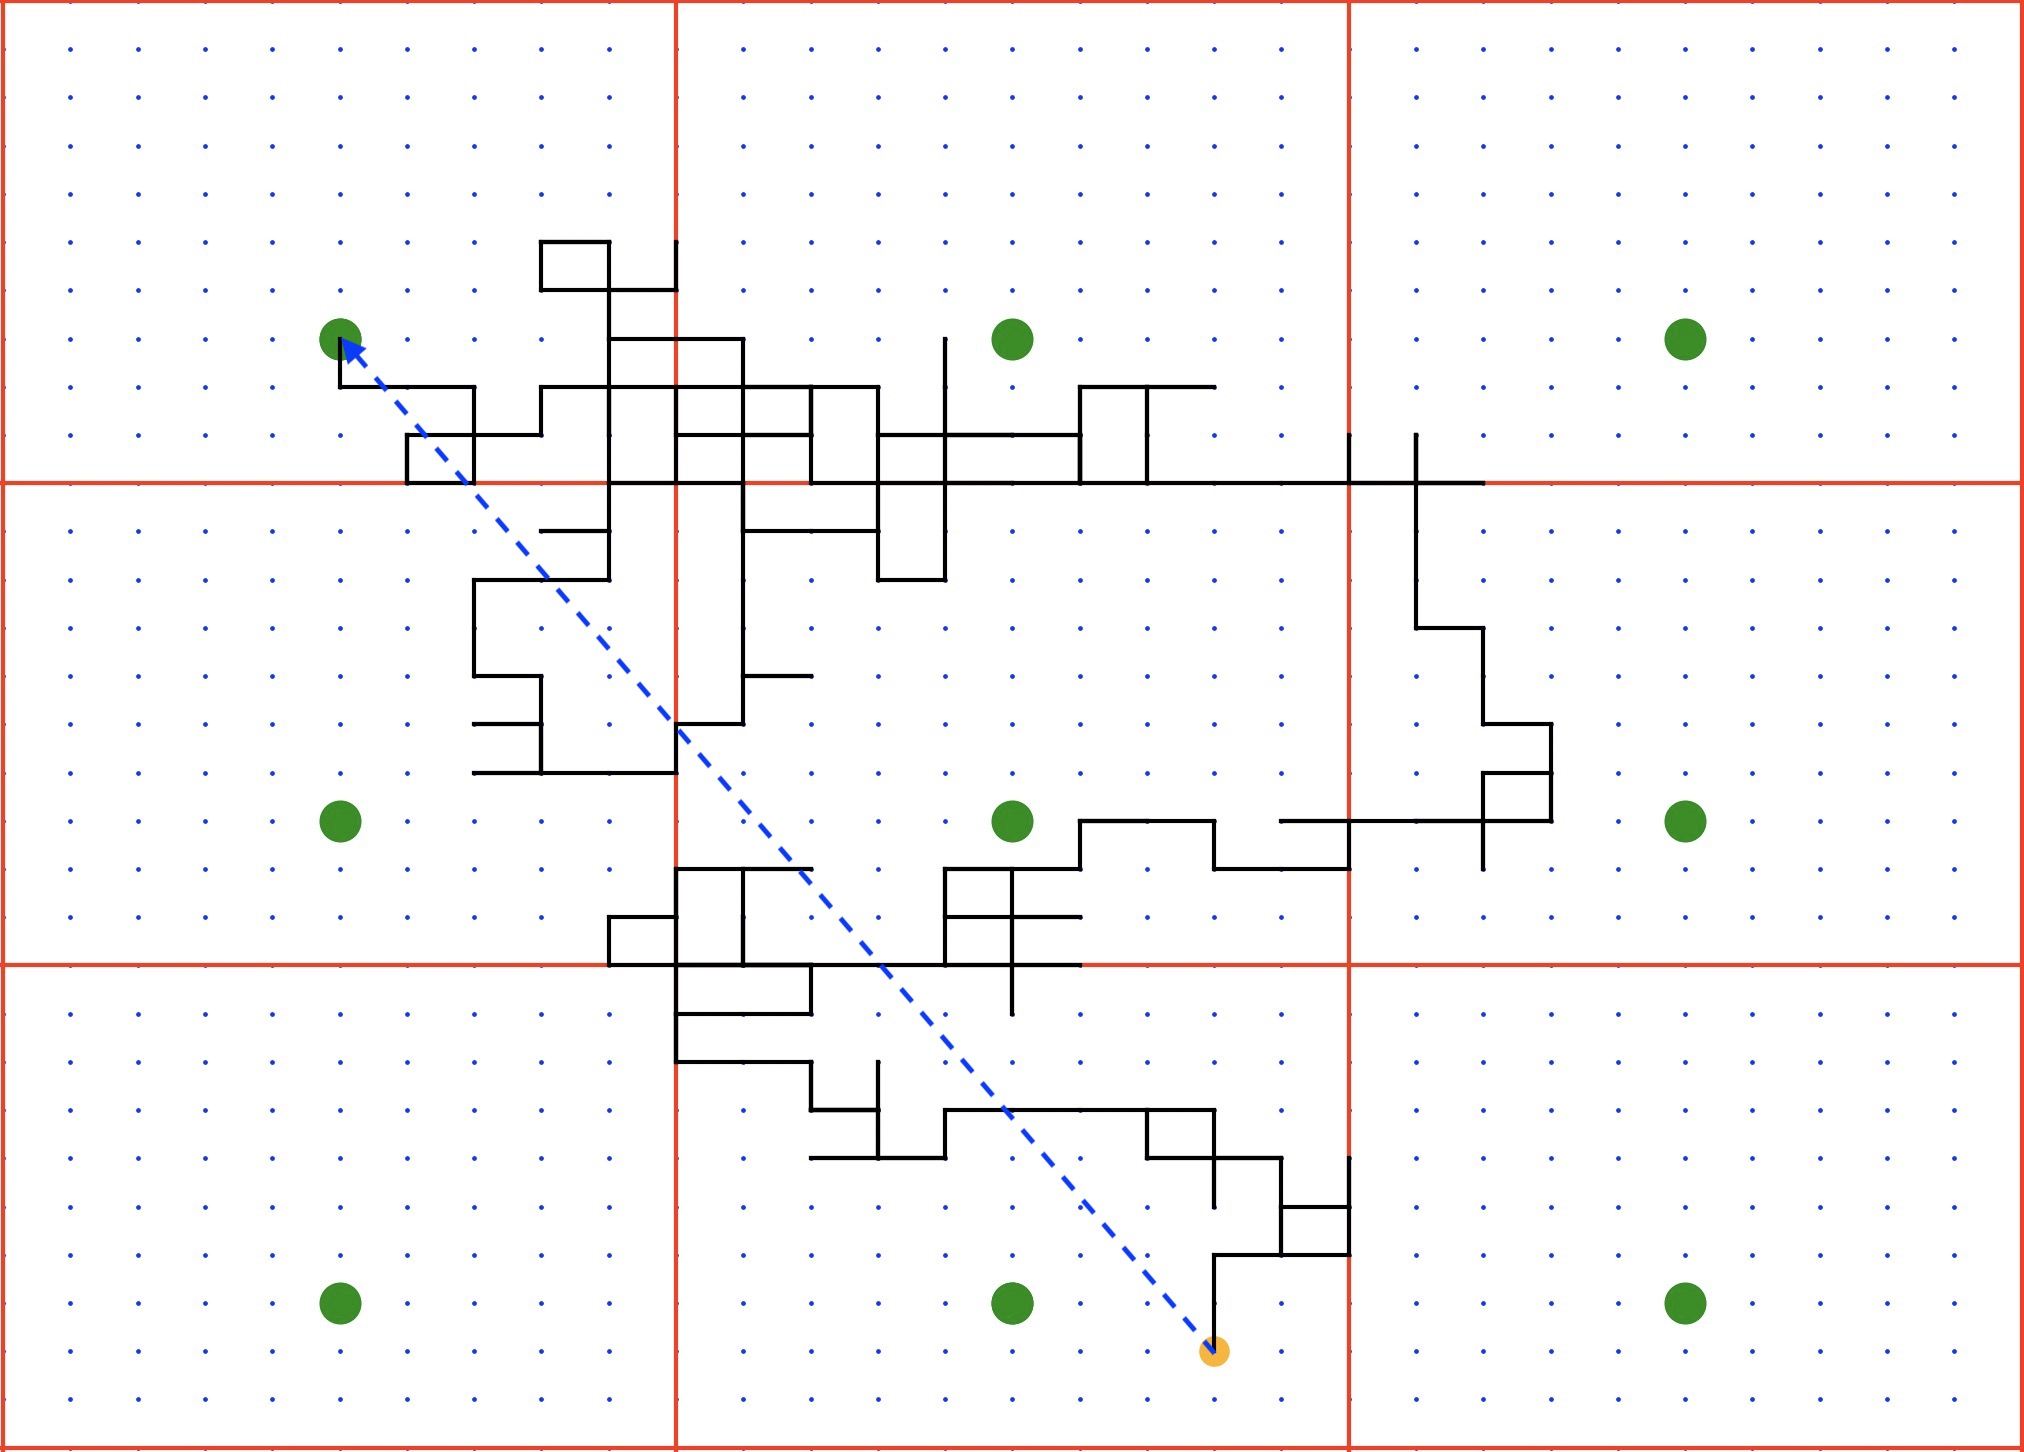
\includegraphics[width=\textwidth]{lrw_perodic_bc.png}
                   \caption{This plane is constructed by choosing a
                     primitive cell with four red sides and a green
                     point and replicating it infinitely to tile the
                     whole $2-$ dimensional space. Moreover, there has
                     no overlaps and voids between copies of the
                     cell. A particle initially started LRWs from the
                     orange site and be absorbed by any of the green
                     points.  To ensure smoothness and consistency, if
                     the particle leaves the cell through one edge, it
                     will appear in the adjacent cell with the same
                     velocity. The black line segments show the
                     particle's random trajectories, and the length of
                     the blue dotted arrow is defined as its
                     displacement.}
                   \label{fig:pbc_lrws}
                 \end{figure}

                 \par
                 
                 In this thesis, periodic boundary conditions (PBCs)
                 are employed to minimize the influence of images'
                 edges. Fig.~\ref{fig:pbc_lrws} is a simplest example
                 of implementing PBCs in the Euclidean plane $E^2$ and
                 tracks the trajectory of a particle undergoing LRWs.
               
               \item Absorbing boundary condition on the boundary of the target shape.
             \end{itemize}
       \end{itemize}
       

   \subsubsection{Survival Function $S_{\Omega}(d)$}

       
